  \documentclass[xcolor=x11names,compress, 24pt]{beamer}
 %\documentclass[handout, t,xcolor=x11names,compress]{beamer}
 %% General document %%%%%%%%%%%%%%%%%%%%%%%%%%%%%%%%%%
 \usepackage{graphicx}
 \usepackage{tikz}
 \usetikzlibrary{arrows,shapes,snakes,automata,backgrounds}
 \usetikzlibrary{decorations.fractals}
 \usetikzlibrary{calc,through,backgrounds}
 \usepackage{graphics}
 \usepackage{setspace} 
 \usepackage{array, multirow}
 \usepackage{latexsym}
 \usepackage{qtree}
 \usepackage{beamerthemesplit}
 \usepackage{algorithmic}
 \usepackage{wrapfig}
 \usepackage{sidecap}
 \usepackage{apalike}
 %%%%%%%%%%%%%%%%%%%%%%%%%%%%%%%%%%%%%%%%%%%%%%%%%%%%%%
 
 \setbeamercolor{math text}{fg=blue!80!black}
 \setbeamercolor{normal text}{fg=blue!80!blue}
 
 \usepackage{supertabular,tabularx}
 \usepackage{listings}
 \usepackage{verbatim}
 \usepackage{color}
 \usepackage{setspace}
 %\usepackage{drop}
 
 
 
 
 %% Beamer Layout %%%%%%%%%%%%%%%%%%%%%%%%%%%%%%%%%%
 %\useoutertheme[subsection=false,shadow]{miniframes}
 %\useinnertheme{default}
 % \usecolortheme{seahorse}
 
 \usetheme{AnnArbor}
 %\useinnertheme[subsection=false,shadow]{rounded}
 %\useoutertheme{infolines}
 \usecolortheme{seahorse}
 \usefonttheme{serif,professionalfonts}
 %\usefonttheme{platino}

 
 \setbeamercolor{header}{fg=white,bg=DeepSkyBlue4}
 \setbeamercolor{frametitle}{bg=white,fg=DeepSkyBlue4}%, fontface=bf}
 \setbeamercolor*{section}{fg=white,bg=DeepSkyBlue4}%, fontface=bf}
 \setbeamercolor{title}{fg=white,bg=DeepSkyBlue4}
 \setbeamercolor{item}{fg=DeepSkyBlue4}
 \setbeamercolor*{lower separation line head}{bg=DeepSkyBlue4} 
 \setbeamercolor*{normal text}{fg=black,bg=white} 
 \setbeamercolor*{alerted text}{fg=red} 
 \setbeamercolor*{example text}{fg=black} 
 \setbeamercolor*{structure}{fg=black} 
 \setbeamercolor*{math text}{fg=blue!80!black}
 \setbeamercolor*{palette tertiary}{fg=black,bg=black!10} 
 \setbeamercolor*{palette quaternary}{fg=black,bg=black!10} 
 
  \newcommand{\rd}[1]{ \textcolor{red}{\textbf{#1}}}
 \newcommand{\bl}[1]{ \textcolor{DeepSkyBlue4}{\textbf{#1}}} 
 
 
 \setbeamerfont{title like}{shape=\scshape, series=\bfseries}
 \setbeamerfont{frametitle}{shape=\scshape, series=\bfseries}
 \setbeamerfont{normal text}{shape=\itshape, series=\bfseries}
 \setbeamerfont{item}{series=\bfseries}
 
 \definecolor{darkblue}{rgb}{0,0,0.6}
 \setbeamercolor{myfootline1}{fg=white,bg=DeepSkyBlue4}
 \setbeamercolor{myfootline2}{fg=white,bg=DeepSkyBlue4}
 
 \setbeamertemplate{headline}{
 	\leavevmode%
 	\hbox{\begin{beamercolorbox}[wd=.5\paperwidth,ht=2.5ex,dp=1.125ex,leftskip=.3cm,rightskip=.3cm]{myfootline1}%
 			\usebeamerfont{author in head/foot}	\insertsection
 		\end{beamercolorbox}%
 		
 		\begin{beamercolorbox}[wd=.5\paperwidth,ht=2.5ex,dp=1.125ex,leftskip=.3cm,rightskip=.3cm plus1fil]{myfootline2}%
 			\usebeamerfont{author in head/foot}\insertsubsection
 	\end{beamercolorbox}}%
 	\vskip0pt%
 }
 
 \setbeamertemplate{footline}{
 	\leavevmode%
 	\hbox{\begin{beamercolorbox}[wd=.5\paperwidth,ht=2.5ex,dp=1.125ex,leftskip=.3cm,rightskip=.3cm]{myfootline1}%
 			\usebeamerfont{author in head/foot}\insertshortauthor~~\insertshortinstitute
 		\end{beamercolorbox}%
 		
 		\begin{beamercolorbox}[wd=.5\paperwidth,ht=2.5ex,dp=1.125ex,leftskip=.3cm,rightskip=.3cm plus1fil]{myfootline2}%
 			\usebeamerfont{title in head/foot}\insertshorttitle\hfill\insertpagenumber
 	\end{beamercolorbox}}%
 	\vskip0pt%
 	\addtocounter{framenumber}{-1}
 }
 %\setbeamerfont{frametitle}{shape=\scshape,series=\bfseries,size={\fontsize{18}{36}}}
 
 
 \renewcommand{\(}{\begin{columns}}
 \renewcommand{\)}{\end{columns}}
\newcommand{\<}[1]{\begin{column}{#1}}
\renewcommand{\>}{\end{column}}


\usepackage{xpatch}
\setlength{\columnsep}{1cm}


\xpatchcmd{\itemize}
{\def\makelabel}
{\usebeamertemplate{itemize body}\def\makelabel}
{}{}


\xpatchcmd{\description}
{\def\makelabel}
{\usebeamertemplate{description body}\def\makelabel}
{}{}


\xpatchcmd{enumerate}
{\def\makelabel}
{\usebeamertemplate{enumerate body}\def\makelabel}
{}{}
\defbeamertemplate*{itemize body}{default}{
\setlength{\itemsep}{2cm}%
} % default is doing nothing

\setbeamertemplate{itemize body}{%
\setlength{\itemsep}{0.2cm}%
}

\setbeamertemplate{description body}{%
\setlength{\itemsep}{0.2cm}%
}

\setbeamertemplate{enumerate body}{%
\setlength{\itemsep}{0.2cm}%
}

\setbeamercovered{transparent}


\definecolor{dkgreen}{rgb}{0,0.6,0}
\definecolor{gray}{rgb}{0.5,0.5,0.5}
\definecolor{mauve}{rgb}{0.58,0,0.82} 
\definecolor{verylightgray}{rgb}{0.95,0.95,0.95}

%%%%%%%%%%%%%%%%%%%%%%%%%%%%%%%%%%%%%%%%%%%%%%%%%%
% Define block styles
\tikzstyle{decision} = [diamond, draw, fill=blue!20, text width=4.5em, text badly centered, node distance=3cm, inner sep=0pt]
\tikzstyle{block} = [rectangle, draw, fill=blue!20,  text width=5em, text badly centered, rounded corners, minimum height=2em]
\tikzstyle{block1} = [rectangle, draw, fill=blue!20, text badly centered, rounded corners,]
\tikzstyle{redblock} = [rectangle, draw, fill=red!20, text badly centered, rounded corners]

\tikzstyle{line} = [draw, -latex']
\tikzstyle{cloud} = [ellipse,fill=red!20, node distance=2cm, text width=5em, text badly centered, minimum height=2em]
\tikzstyle{info} = [ellipse, node distance=4cm, text width=5em, text badly centered, minimum height=2em]
\tikzstyle{prg} = [ ellipse, node distance=4cm, minimum height=2em]
\tikzstyle{prg2} = [ ellipse, node distance=2cm, minimum height=2em]
\tikzstyle{prg3} = [ ellipse, node distance=2cm,text width=5em, text badly centered,  minimum height=2em]
\tikzstyle{elp} = [draw,ellipse, node distance=2cm, minimum height=2em]
\tikzstyle{int}=[draw, fill=blue!20, minimum size=2em]
\tikzstyle{init} = [pin edge={to-,thin,black}] 
%%%%%%%%%%%%%%%
%\usefonttheme{professionalfonts}
\usefonttheme{professionalfonts}
\logo{
\includegraphics[height=0.075\paperheight]{cu}} 


\title{\sc Introduction to Data Engineering}
\subtitle{Lecture  1}
\author{Rokan U. Faruqui }
\author{\sc Rokan Uddin Faruqui }

\institute[CSE, CU]{Associate Professor \\ Dept of Computer Science and Engineering \\ University of Chittaong, Bangladesh\\ Email: \textit{rokan@cu.ac.bd}}
\date{} %Mon, July 01, 2019}

%\begin{comment}
\AtBeginSection[]
{
	\begin{frame}<beamer>{Outline}
	\tableofcontents[currentsection,currentsubsection]
\end{frame}
}

\AtBeginSubsection[]
{
\begin{frame}<beamer>{Outline}
\tableofcontents[currentsection,currentsubsection]
\end{frame}
}


%\end{comment}
\begin{document}

\begin{frame}[plain]
\titlepage
\end{frame}

\begin{frame}{Outline}
\tableofcontents
\end{frame}
 \section{Data Engineer vs Data Scientist}
 \begin{frame}{Data Engineer}
 \begin{itemize}
 	\item Data Engineers are the link between the management's data strategy and the data scientists that need to work with data.  \vspace{.25cm}
 	
    \item What they do is building the platforms that enable data scientists to do their magic.
 	
 	 
 \end{itemize}
 \end{frame}


 \begin{frame}{Data Engineer}
	\begin{itemize}
		 
		\item These platforms are usually used in five different ways:  \vspace{.25cm}
		
		\begin{enumerate}
			\item Data ingestion and storage of large amounts of data \vspace{.25cm}
			
			\item Algorithm creation by data scientists  \vspace{.25cm}
			
			\item Automation of the data scientist's machine learning models and algorithms for production use  \vspace{.25cm}
			
			\item Data visualization for employees and customers  \vspace{.25cm}
			
			\item Most of the time these guys start as traditional solution architects for systems that involve SQL databases, web servers, SAP installations and other "standard"  systems.  \vspace{.25cm}
		\end{enumerate}

	\end{itemize}
\end{frame}

\begin{frame}{Data Engineer}
	\begin{itemize}
		\item But to create big data platforms the engineer needs to be an expert in specifying, setting up and maintaining big data technologies like: \textbf{Hadoop, Spark, HBase, Cassandra, MongoDB, Kafka, Redis} and more. \vspace{.25cm}
		
		\item What they also need is experience on how to deploy systems on cloud infrastructure like at \textbf{Amazon} or \textbf{Google} or on-premise hardware. \vspace{.25cm}
	\end{itemize} 
\end{frame}

\begin{frame}{Data Scientist}
	\begin{itemize}
		\item use linear algebra and multivariable calculus to create new insight from existing data.
	\end{itemize}
\end{frame}

\begin{frame}{Data Scientist: Case Study}

\begin{itemize}
\item An industrial company produces a lot of products that need to be tested before shipping. \vspace{.25cm}

\item 	Usually such tests take a lot of time because there are hundreds of things to be tested. All to make sure that your product is not broken. \vspace{.25cm}

\item 	Wouldn't it be great to know early if a test fails ten steps down the line? If you knew that you could skip the other tests and just trash the product or repair it. \vspace{.25cm}

\item 	That's exactly where a data scientist can help you, big-time. This field is called predictive analytics and the technique of choice is machine learning.  \vspace{.25cm}
\end{itemize}

\end{frame}


\begin{frame}{Data Scientist: Case Study}
	\begin{itemize}
		\item 	You feed an algorithm with measurement data. It generates a model and optimises it based on the data you fed it with. 
		
		\item That model basically represents a pattern of how your data is looking. You show that model new data and the model will tell you if the data still represents the data you have trained it with. 
		
		\item This technique can also be used for predicting machine failure in advance with machine learning. Of course the whole process is not that simple.
		
		\item 	The actual process of training and applying a model is not that hard. A lot of work for the data scientist is to figure out how to pre-process the data that gets fed to the algorithms.
		 
	\end{itemize}
\end{frame}

\begin{frame}{Machine Learning Pipeline}
	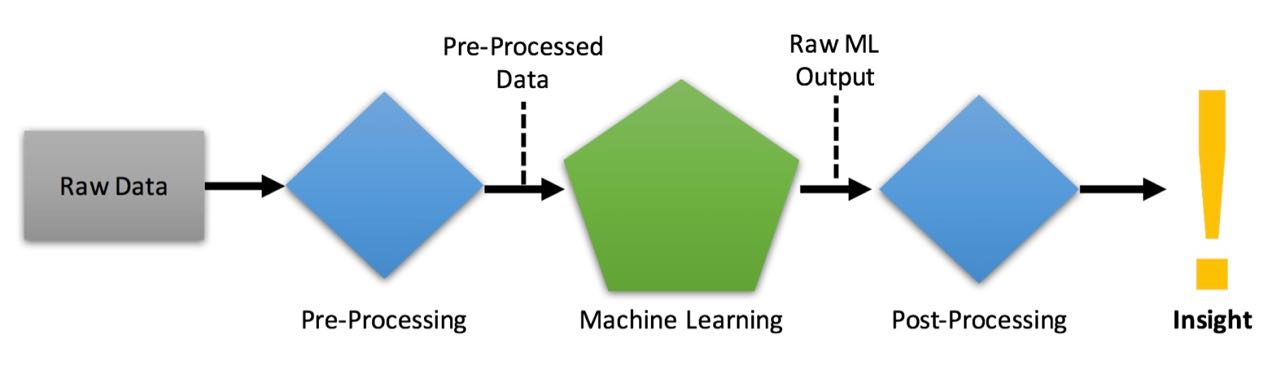
\includegraphics[scale=.25]{Machine-Learning-Pipeline}
\end{frame}

\begin{frame}{Data Scientist: Case Study}
	\begin{itemize}
	 
		
		\item 	In order to train an algorithm you need useful data. If you use any data for the training the produced model will be very unreliable.
		
		\item 	An unreliable model for predicting machine failure would tell you that your machine is damaged even if it is not. Or even worse: It would tell you the machine is ok even when there is a malfunction.
		
		\item 	Model outputs are very abstract. You also need to post-process the model outputs to receive the outputs you desire.
	\end{itemize}
\end{frame}




\begin{frame}{Machine Learning Workflow}
	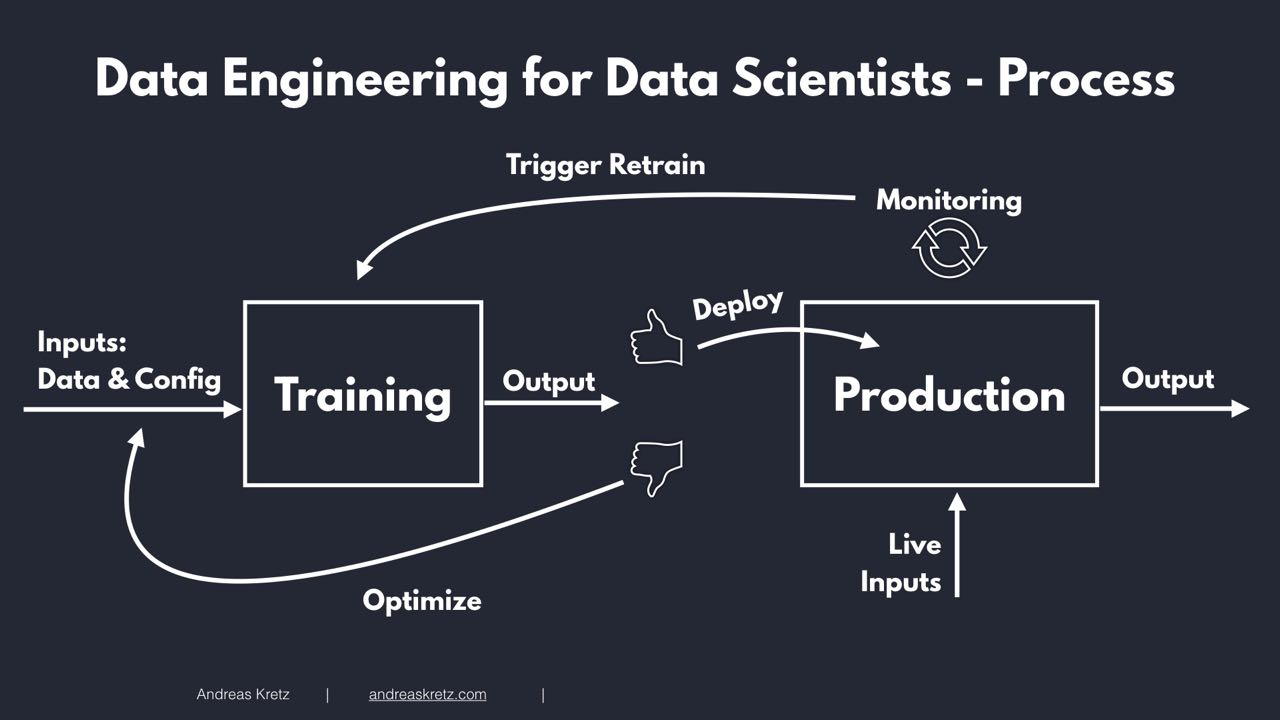
\includegraphics[scale=.25]{Machine-Learning-Workflow}
\end{frame}

\begin{frame}{Machine Learning Model}
	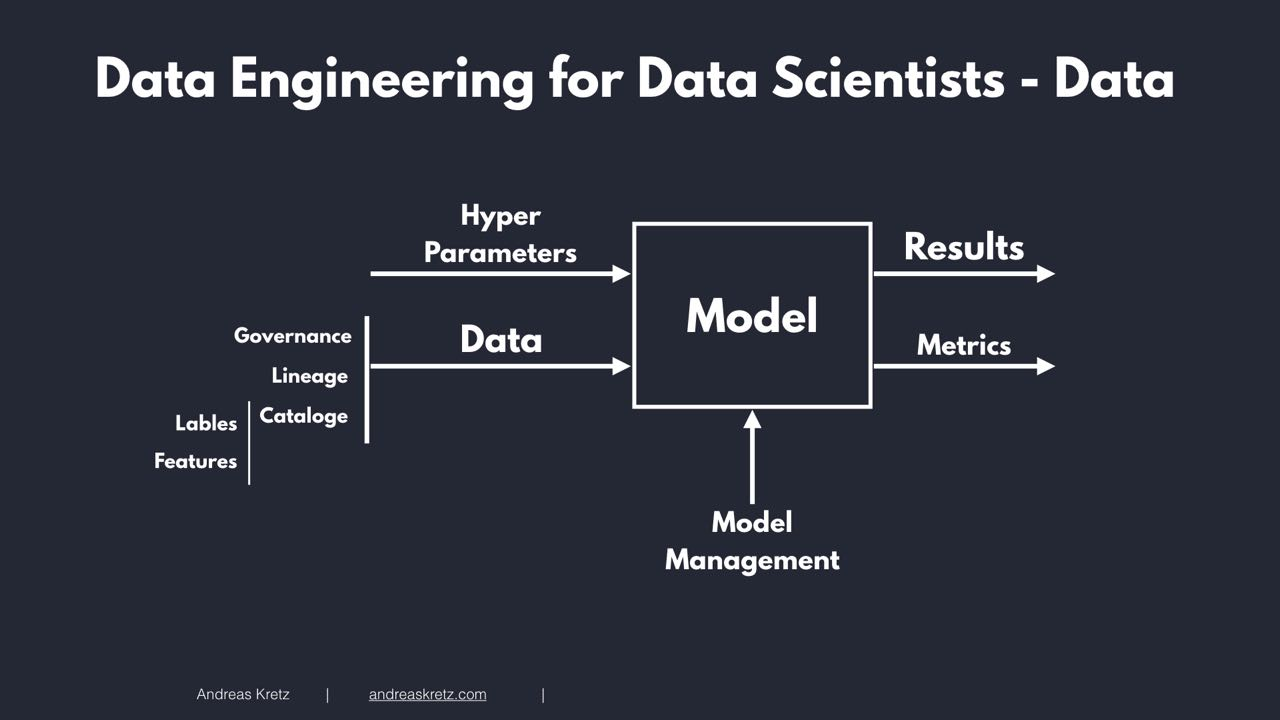
\includegraphics[scale=.25]{Machine-Learning-Model}
\end{frame}


\begin{frame}{Data Science Platform}
	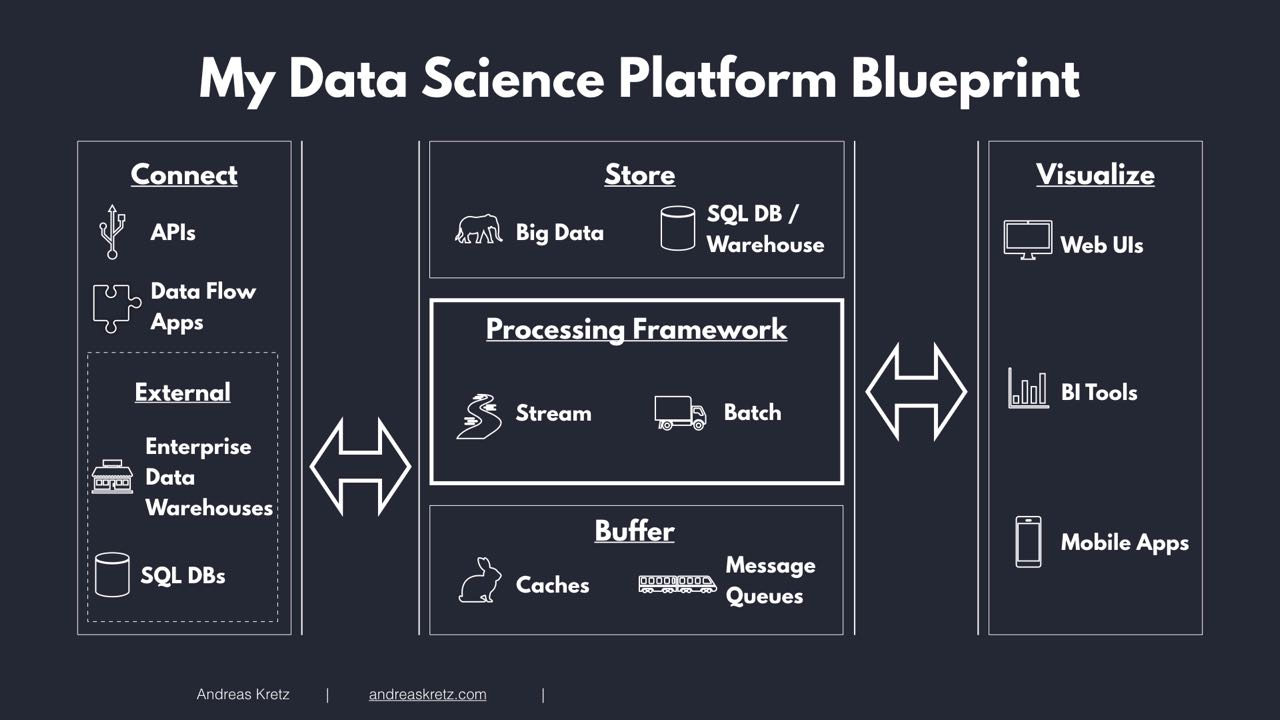
\includegraphics[scale=.25]{Data-Science-Blueprint-New}
\end{frame}


\end{document}